
\chapter{Background Theory}

\label{ch:background}

\section{The Description of Perfect Periodic Crystal Structures}
Theoretical models of crystalline solids are based around the existence of translational symmetry in a crystal lattice such that the lattice can be constructed from periodically repeating a unit cell of atoms. The Bravais lattice specifies the periodic array in which the repeated units of the crystal are arranged. A crystal lattice can therefore be described by its underlying Bravais lattice and the arrangement of atoms, ions or molecules within a particular unit cell, i.e. the basis \cite{AshcroftMermin2}. This principle is used in a number of ways during this study. Firstly, this process is performed on a finite scale to construct a 64 atom supercell of CZTS from the 8 atom primitive unit cell for use in density functional theory (DFT) calculations. This process is discussed further in section \ref{supercell_section} and an outline of DFT is given in section \ref{DFT_section}. The principle is also used in the DFT calculations through the implementation of periodic boundary conditions to simulate an infinite, bulk system using only a finite supercell.\\
 
Another important concept in the theoretical modelling of periodic structures is reciprocal space and the reciprocal lattice. 
Converting to reciprocal space enables the description of periodic features with a longer-range periodicity than the unit cell in real space, such as the motion of electrons in a crystal and phonons.
In the same way that any quantity that varies with time can be described as a sum of Fourier components in the frequency domain; the spatial properties of a crystal can be described as a sum of components in Fourier space, otherwise known as reciprocal space or \textit{k}-space. The reciprocal lattice of a perfect single crystal is an infinite periodic 3D array of points whose spacings are inversely proportional to the distances between the planes in the lattice in real space. Vectors in real space have dimensions of length, whereas vectors in reciprocal space have dimensions of length$^{-1}$. This can therefore be compared directly to the wavevector $ \left(k  = \frac{2\pi}{\lambda} \right)$ of an excitation such as a phonon or a moving electron and multiplication of each coordinate of the reciprocal lattice by $\hbar$ converts reciprocal space into momentum space as for a quantised wave $\mathbf{p} = \hbar \mathbf{k}$ \cite{Blakemore1}. \\ 

The Wigner-Seitz primitive cell is the most common choice of primitive cell with the full symmetry of the Bravais lattice. It represents the region of space around a lattice point  that is closer to that point than to any other lattice point. For example, figure \ref{Wigner-Seitz}a shows the truncated octahedron that is the Wigner-Seitz cell for a body-centred cubic (bcc) lattice \cite{AshcroftMermin2}.
The first Brillouin zone is the Wigner-Seitz primitive cell of the reciprocal lattice. The reciprocal of the bcc lattice is face-centred cubic (fcc), therefore the first Brillouin zone of  of the bcc lattice is the fcc Wigner-Seitz primitive cell as shown in figure \ref{Wigner-Seitz}b \cite{AshcroftMermin3}. As the full symmetry of the reciprocal lattice is contained within the first Brillouin zone, it is only necessary to sample \textit{k}-points within this single unit cell of the reciprocal lattice when calculating the electronic ground state of a periodic structure.
\begin{figure}[h!]
  \centering
    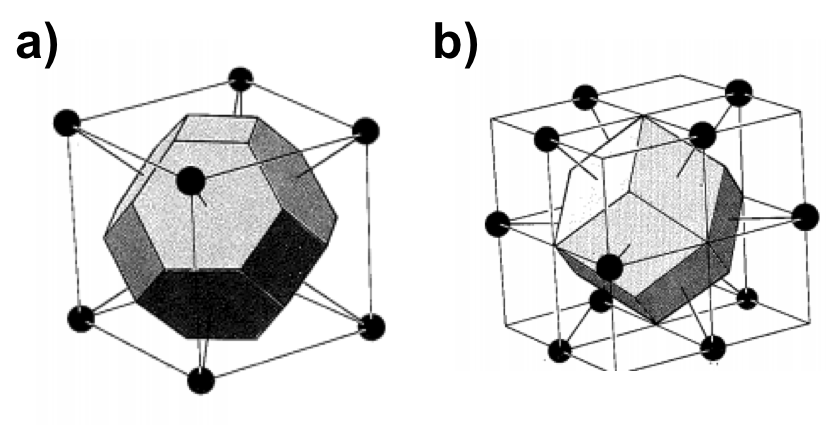
\includegraphics[width=0.5\textwidth]{figures/Wigner-Seitz.png}
    \caption{The Wigner-Seitz cell for the body-centred cubic Bravais lattice where there is a lattice point at its centre and on each vertex. The hexagonal faces bisect the lines joining the central point to the points on the vertices. The square faces bisect the lines joining the central point to the central points in each of the six neighbouring cubic cells. Figure taken from reference \citenum{AshcroftMermin2}.}
  \label{Wigner-Seitz}
\end{figure}
 
Another important aspect of the theoretical modelling of periodic structures for this 
study is the motion of an electron in the periodic structure. In the band theory of 
solids, the energy of a single electron in a perfect crystal is described by the one-electron 
Schr{\"o}dinger equation, shown in equation \ref{single_SE}. Scattering caused by phonons or defects are introduced afterwards as a perturbation. The first term in equation \ref{single_SE} is the kinetic 
energy of the electron, V(\textbf{r}) is the effective non-zero periodic potential energy experienced by 
the electron in the crystal, $\psi$ is the electron wavefunction and  $\epsilon$ is the 
eigenenergy of the electron. In band theory, it is assumed that for any electron everything else in the crystal can be represented by the effective potential energy, V(\textbf{r}) \cite{Blakemore2}.
\begin{equation} \label{single_SE}
\left[ \left(-\frac{\hbar^2}{2m}\right)\nabla^2 + V(\mathbf{r})\right]\psi = \epsilon \psi 
\end{equation}

The spatial dependence of the potential experienced by an outer electron in a crystal 
for multi-electron systems was considered by Felix Bloch. He determined that the total 
potential is the sum of two parts. Firstly, the electrostatic potential due to the array 
of atomic cores. For a perfect lattice this should have the translational periodicity of 
the lattice. Secondly, the potential due to all other electrons. Bloch assumed that the 
charge density would have the same long-term average value in every unit cell of the 
crystal and therefore would be periodic. Bloch's theorem states that the wavefunction 
which satisfies equation \ref{single_SE} subject to a periodic potential should be of 
the form shown in equation \ref{bloch}, where $U_k(\mathbf{r})$ is some function 
(depending on the value of the wavevector, \textbf{k}) that also has the complete 
periodicity of the lattice and \textbf{k} is confined to the first Brillouin zone \cite{Blakemore2}.
\begin{equation} \label{bloch}
\psi_k(\mathbf{r}) = U_k(\mathbf{r}) e^{i\mathbf{k \cdot r}} 
\end{equation}
\begin{figure}[h!]
  \centering
    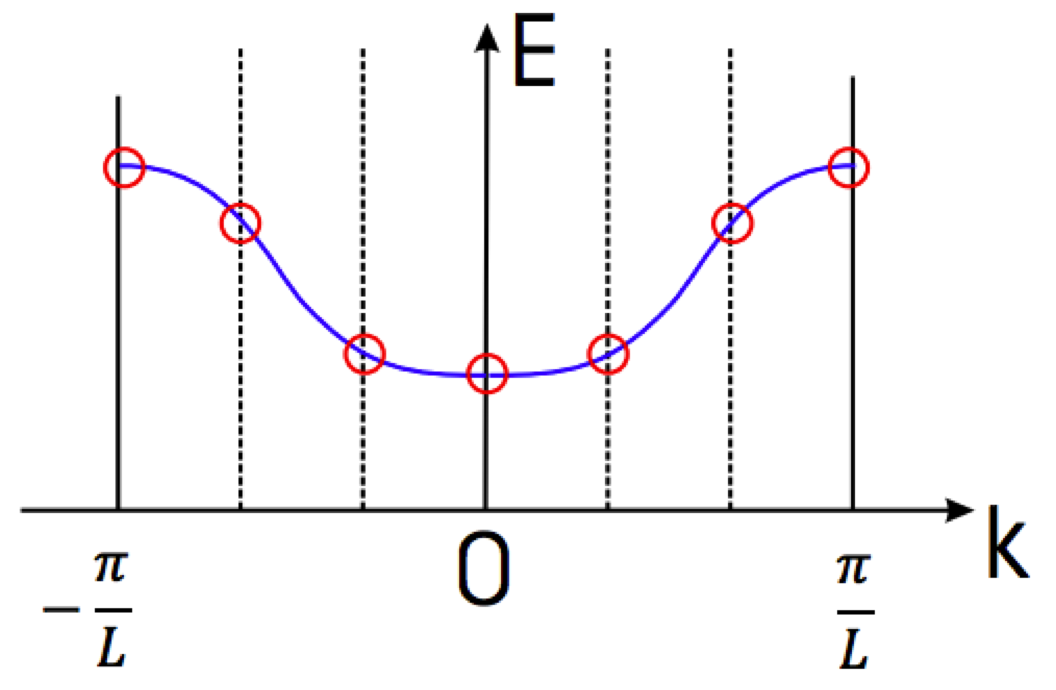
\includegraphics[width=0.4\textwidth]{figures/energy_dispersion.png}
    \caption{The energy dispersion relation for electrons moving in a crystal, illustrating how the function can be approximately represented by a finite number of \textit{k}-points, which form an equally-spaced mesh. Figure adapted from reference \citenum{vasp-slides}.}
  \label{energy_dispersion}
\end{figure}
Each electron occupies a state of definite $\mathbf{k}$. Therefore, an infinite number of electrons within the solid would result in an infinite number of \textit{k}-points. At each \textit{k}-point, only a finite number of the available energy levels will be occupied. Therefore only a finite number of electrons need to be considered but at an infinite number of \textit{k}-points. In practise, all of these \textit{k}-points are not considered. 
Electron wavefunctions will be almost identical for values of $\mathbf{k}$ that are sufficiently close, so the wavefunctions over a region of reciprocal space can be represented by considering the wavefunction at a single \textit{k}-point. It is therefore sufficient to consider the electronic states at a finite number of \textit{k}-points in order to determine the ground state energy of the solid. This approximation is illustrated in figure \ref{energy_dispersion}. Using Bloch's Theorem therefore has enabled the ground state energy to be determined by considering only the number of electrons in the unit cell at a finite number of \textit{k}-points, which are chosen to sample the Brillouin zone appropriately. The choice here is a balance between more \textit{k}-points for a more accurate representation of the Brillouin zone and fewer \textit{k}-points to reduce the computational expense of the calculation \cite{bloch-thesis}.



\section{Crystal Imperfections \& Disorder}
\begin{itemize}
\item Notes from A. Guinier 'X-Ray Diffraction' CH6 + Ziman
\item Mention many types of disorder possible for multicomponent, especially for multi-component, compound semiconductor. e.g. of many types of possible defects for CdTe from Ken's work - and that's just binary!
\item Extended defects usually detectable? 
\end{itemize}





\section{Band Theory \& Band Structure of Semiconductors}\label{band_theory}
See MRes2 report + use e.g. of Si, state that early figure is a simplification and use to discuss why Si is not ideal from indirect band gap, use rough calc from lecture



The band theory of solids provides a means to explain the difference in the electrical conductivity of conductors, semiconductors and insulators. Electrons bound to an atom have a number of possible discrete energy levels. When a large number of atoms are brought together to form a solid, it becomes impossible to assign individual electrons to individual atoms. Instead, the electrons are considered to be shared amongst the atomic nuclei. However, a consequence of this sharing would be a large number of electrons occupying the same energy state, which violates the Pauli Exclusion Principle. The original discrete energy levels therefore are broadened into bands. The new energy levels are so closely spaced that they are considered to be a quasi-continuous band of allowed energies. The series of bands of allowed energies in a semiconductor or insulator are separated by bands of forbidden energy, known as the band gap, E$_g$, of the material \cite{dielectric1}. In the simplest model, the upper energy band (the conduction band) is separated from the lower energy band (the valence band) by a constant band gap. This is called the flat band model. In real structures, the band architecture is more complicated than this simple model\cite{Tilley}.\\

The concept of the energy band model of a solid emerges from considering the behaviour of electrons in a periodic crystal lattice, but cannot be understood in terms of classical physics alone. Instead, the electron must be considered in terms of wave-mechanical terms as a wave propagating in a periodic structure with diffraction and interference effects  \cite{small_semiconductor1}.
In the band theory of 
solids, the energy of a single electron in a perfect crystal is described by the one-electron Schr{\"o}dinger equation, shown in equation \ref{single_SE}. The first term in equation \ref{single_SE} is the kinetic 
energy of the electron, V(\textbf{r}) is the effective non-zero periodic potential energy experienced by 
the electron in the crystal, $\psi$ is the electron wavefunction and  $\epsilon$ is the eigenenergy of the electron. In band theory, it is assumed that for any electron, everything else in the crystal can be represented by the effective potential energy, V(\textbf{r}) \cite{Blakemore2}.
\begin{equation} \label{single_SE}
\left[ \left(-\frac{\hbar^2}{2m}\right)\nabla^2 + V(\mathbf{r})\right]\psi = \epsilon \psi 
\end{equation}
The spatial dependence of the potential experienced by an outer electron in a crystal for multi-electron systems was considered by Felix Bloch. He determined that the total potential is the sum of two parts. Firstly, the electrostatic potential due to the array of atomic cores. For a perfect lattice this should have the translational periodicity of the lattice. Secondly, the potential due to all other electrons. Bloch assumed that the charge density would have the same long-term average value in every unit cell of the crystal and therefore would be periodic. Bloch's theorem states that the wavefunction which satisfies equation \ref{single_SE} subject to a periodic potential should be of the form shown in equation \ref{bloch}, where $U_k(\mathbf{r})$ is some function 
(depending on the value of the wavevector, \textbf{k}) that also has the complete 
periodicity of the lattice and \textbf{k} is confined to the first Brillouin zone \cite{Blakemore2}.
\begin{equation} \label{bloch}
\phi_k(\mathbf{r}) = U_k(\mathbf{r}) e^{i\mathbf{k \cdot r}} 
\end{equation}
\begin{equation} \label{bloch_sum}
\psi_k(\mathbf{r}) = \sum_k A_k \phi_k(\mathbf{r}) = \sum_k A_kU_k(\mathbf{r}) e^{i\mathbf{k \cdot r}} 
\end{equation}
Due to the translational symmetry of a crystal lattice, an eigenfunction of the one-electron Schr{\"o}dinger equation can be expressed as a sum of Bloch functions such as that shown in equation \ref{bloch}, as shown in equation \ref{bloch_sum}. The one-electron wavefunctions therefore can be indexed by constants \textbf{k}, which are the wave vectors of the plane waves forming the `backbone' of the Bloch function. A plot of the electron eigenenergies from equation \ref{single_SE} versus \textbf{k} is known as the electronic band structure of the crystal \cite{fund_semi}.\\

\begin{figure}[h!]
  \centering
    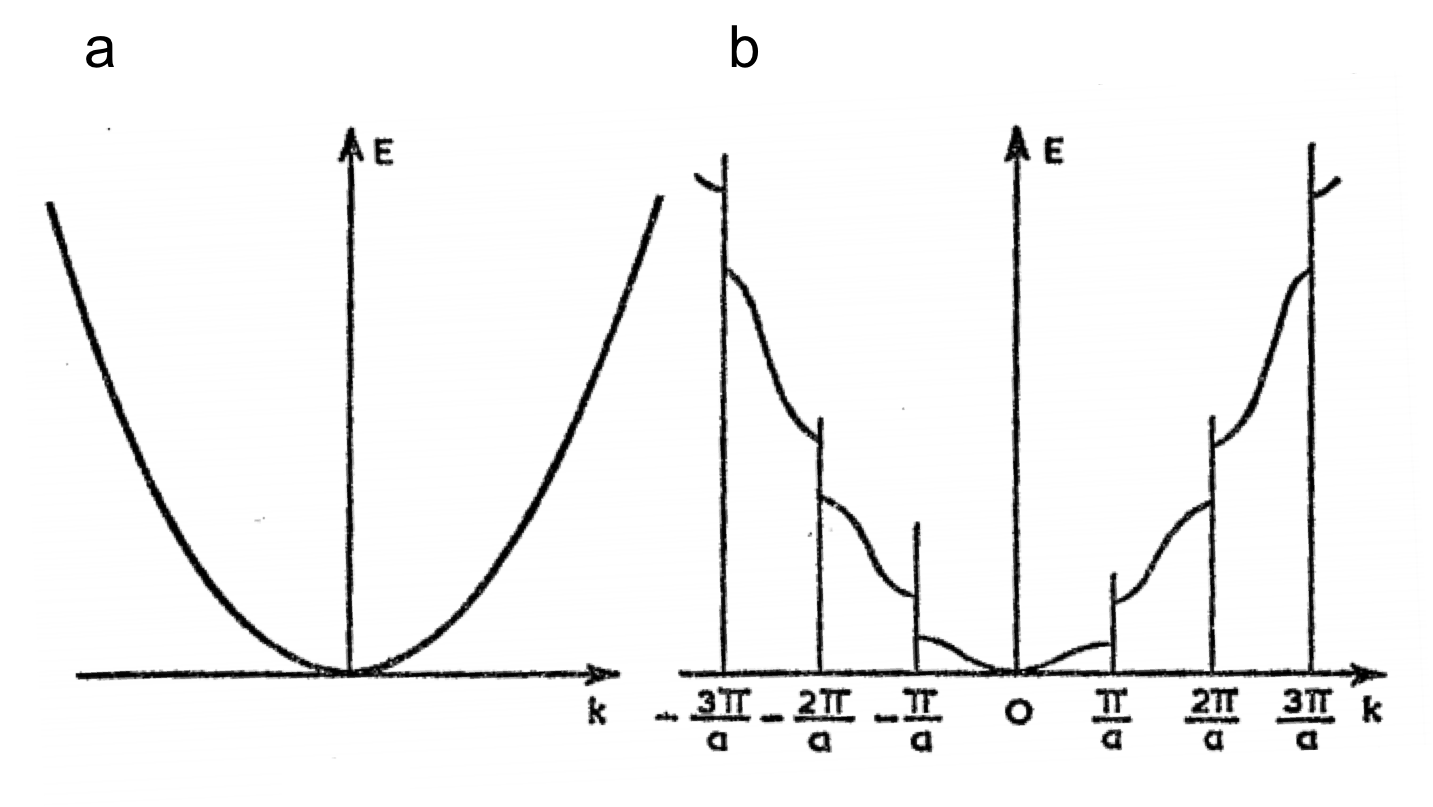
\includegraphics[width=0.7\textwidth]{figures/bs1.png}
    \caption{Energy-wave vector diagrams: (a) the free electron parabola, (b) modification due to a periodic crystal lattice. Figure taken from reference \citenum{small_semiconductor1}.}
  \label{bs1}
\end{figure}

The introduction of a medium with a discrete structure, such as a crystal lattice, has a profound effect on the dispersion relation of the waves. The energy dispersion relation of a free electron and that in a periodic crystal lattice is shown in figure \ref{bs1}. A periodic medium does not completely suppress the propagation of waves, as would be expected  in disordered or amorphous structures, but they do however introduce limiting frequencies and wavelengths for the propagation, followed by cut-off regions. The lower limit of the wavelength is set by the lattice spacing, a, giving an upper limit of the wave vector, \textbf{k}, of $\frac{\pi}{a}$. As figure \ref{bs1} shows, the parabola of the free electron in modified in a periodic crystal by the introduction of discontinuities at values of \textbf{k} corresponding to multiples of $\frac{\pi}{a}$. The appearance of such energy gaps implies that electrons in a periodic crystal may only have kinetic energies corresponding to certain bands, whilst being free to propagate in the lattice \cite{small_semiconductor2}.\\

The energy band model has been successful in explaining many aspects of the behaviour of solids and a large amount of experimental data collected has supported the theoretical predictions made using the model. Its main drawback however is that is assumes a perfect, or nearly perfect, crystal lattice. It applies well to single crystals and polycrystalline substances, but cannot be applied to materials that are amorphous or heavily disordered so that the structure deviates significantly from the periodicity of the crystal \cite{small_semiconductor1}. Low concentrations of impurities and defects can be modelled by considering, for example, the introduction of additional donor and acceptor energy levels within the band gap of a material and the scattering of electrons and holes in the solid. However, at higher defect concentrations the band profile can be modified as shown in figure \ref{bs2} to give rise to conductivity even at temperatures that are too low to produce excitation of carriers into the free conduction bands, called impurity band conduction \cite{small_semiconductor2}.\\

\begin{figure}[h!]
  \centering
    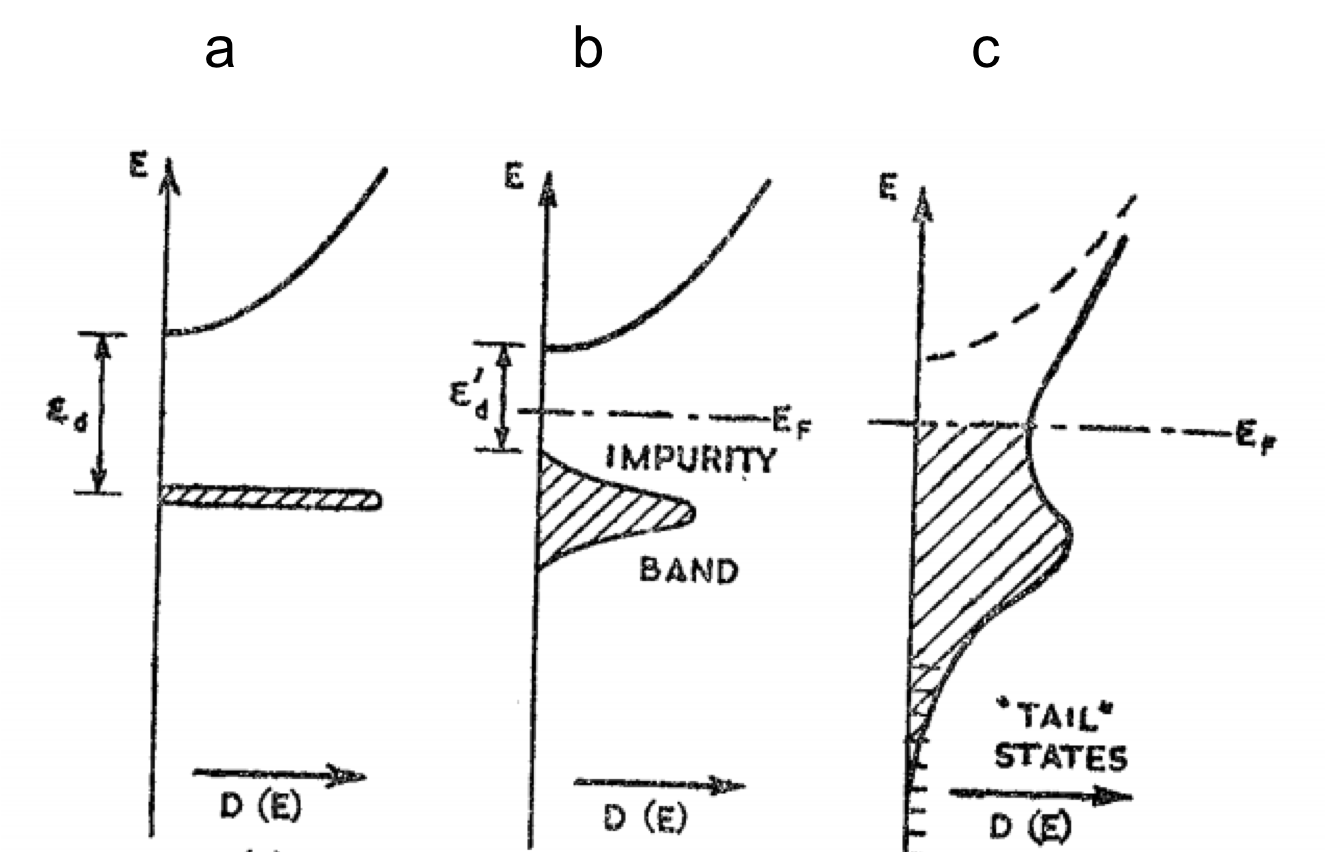
\includegraphics[width=0.7\textwidth]{figures/bs2.png}
    \caption{The influence of increased donor impurity density on the conduction band profile showing low (a), medium (b) and high (c) densities of impurities. Figure taken from reference \citenum{small_semiconductor2}.}
  \label{bs2}
\end{figure}

A useful concept used to simplify the dynamics of an electron in a crystal lattice in the band theory of solids is that of effective mass. The effective mass is a convenient parameter which accounts for the influence of a periodic lattice on a free carrier, enabling an electron in a periodic crystal to be treated as though it were a free particle but with a different mass in calculations of charge transport. Values of effective mass in semiconductors usually vary between 0.01 and 1 times the mass of a free electron and it is determined by the curvature of the energy graph in \textbf{k}-vector space \cite{small_semiconductor2}. The effective mass is a parameter that can influence the efficiency of a solar cell, in particular, the effective mass of holes in the valence band and electrons in the conduction band (i.e. minority charge carriers) are of interest. The mobility of charge carriers is inversely proportional to the effective mass and the mobility of charge carriers in a PV material is important for efficient charge collection \cite{transport}.




\section{Emission Spectroscopies of Semiconductors}\label{PL_section}
Cardona, S7.1 Emission Spectroscopies

Photoluminescence (PL) imaging is becoming a popular method to inspect solar cell materials, it does not require a full functioning device and can be a powerful tool for probing defects in semiconductors \cite{characterization_book, Gerschon}. The PL spectra of \CZTS (CZTS) provides clear evidence of disorder in the material.

Overview of technique, information gained from technique, T dependent PL, PL spectra of CZTS: single crystal and thin film.



\section{Performance Bottlenecks Due to Crystal Imperfections}

\subsection{Impact of Defects and Disorder on Photovoltaic Performance}\label{defects_in_PV}
SRH recomb, GBs, secondary phases, band gap and electrostatic potential fluctuations\\
See CMP lectures on defects + ebook reading material 

\subsection{Band Tailing in Disordered Semiconductors}
Metal disorder in CZTS due to limited cooling/ annealing times, link to Jonathan Scragg's work (years to cool to perfect crystal)

Nelson, pg 65, 3.5.4: heavy doping leading to band tailing

see Pankove + Russian 1970s papers, Urbach tail, fluctuations in electrostatic potential\\
See Urbach tail doc (pg 36) and use Cu/ Zn culprit paper + link to eris

+ see desktop papers from Jarv x2




\section{Novel Optoelectronic Phenomena \& the Possibility of High Performance Solar Cells}


\subsection{Spin Orbit Interaction \& Rashba Splitting}
 see webpages: pg 84 for discussion of effect of SOC on lattice without inversion symmetry!  + useful slide

Look for textbook source?

\subsection{Photovoltaic-Ferroelectric Phenomena}\label{FE_PV_section}

Ferroelectric PV materials are currently receiving a great deal of research interest, however the origin of their PV properties are considered to be unresolved \cite{Rappe}. A large number of theories have been proposed in an attempt to explain the two observed ferroelectric-photovoltaic (FE-PV) phenomena: the bulk PV effect (BPE), also referred to as the photogalvanic effect, and the anomalous PV effect (APE). In the BPE, a direct current appears in a homogeneous medium under uniform illumination and this can occur in all materials without a center of symmetry  \cite{PGE}. Ferroelectric materials exhibit this effect strongly \cite{Rappe} and the first observation of this effect was in 1956 with photovoltages measured in un-doped single crystals of the ferroelectric material BaTiO$_3$ \cite{keith_46}. In the case of the APE, photovoltages have been measured that are orders of magnitude larger than the band gap of the material \cite{keith_54}, but has been observed to disappear when the sample undergoes a phase transition to a paraelectric phase \cite{nonlinear_dielectric}, and so no longer exhibits spontaneous electric polarization. Theories have been developed to explain the FE-PV phenomena based around experimental observations of factors that have been shown to influence the photovoltage of FE-PV devices, such as:  the distance between the two opposite electrodes \cite{rev_28,rev_46}, intensity of incident light \cite{rev_47}, electrical conductivity \cite{Fridkin}, remnant polarization of the
ferroelectric crystals \cite{rev_48}, crystallographic orientation \cite{rev_49}, the dimension or size of the crystals \cite{rev_46, rev_50}, domain walls \cite{rev_30}
and the interface between the FE material and the electrode \cite{rev_37}.\\

Models have been proposed to explain the BPE in ferroelectric materials based upon the built-in asymmetry of non-centrosymmetric crystals. One model is based on asymmetric scattering centres in the materials \cite{PGE}. In non-centrosymmetric crystals, the rate of the generation of charge carriers with momenta $\pm$k can be different due to asymmetric electron-hole scattering. A `ballistic current' can then be generated due to the momentum imbalance \cite{shift_current}.
Another model, the shift current model \cite{shift_current}, has been proposed, which is based on the asymmetry of the electron density \cite{keith}.
Light-induced transitions of charge carriers between bands in reciprocal space are accompanied by asymmetrical shifts in real space between atoms in elementary cells \cite{shift_current}.
Such currents have been demonstrated for a number of materials, such as GaAs \cite{keith_52} and BiFeO$_3$, where this has been demonstrated using both computational \cite{keith_25} and experimental \cite{keith_51} techniques. The shift current model has been used in first principles calculations to reproduce experimental photocurrent direction and magnitude as a function of light frequency resulting from the BPE in BaTiO$_3$\cite{Rappe}. 
The nonlinear dielectric model has also been proposed to explain the BFE effect in (Pb, La)(Zr, Ti)O$_{3}$ (PLZT) ceramics \cite{nonlinear_dielectric}. This material exhibits the photostrictive effect, where strain is induced in the sample by incident light. In this model, the large photovoltage is believed to be due to the nonlinear response of the material to the incident light, which results in an effective DC electric field throughout the ferroelectric material \cite{FE_PV_rev1}.\\

The domain wall theory has been proposed to explain the large generated photovoltages in the APE \cite{domain_wall} and the Schottky-junction effect \cite{schottky_effect} and depolarization field model \cite{screen_effect, depol_model}, also referred to as the screening effect, have been proposed as additional contributions to the large photovoltage. Unlike the BPE, some theories to explain the APE rely on the nano- and microstructure of the material \cite{keith}. The latter two theories are related to the interface between the FE material and an electrode in a FE-PV device, but were originally neglected as the contributions to the photovoltage were believed to be small. However, these effects become more significant in thin-film devices where photovoltages are typically low \cite{FE_PV_rev1}, and thin-films are particularly relevant for PV applications.
The domain wall theory was developed to explain observations of photovoltages in thin films of BiFeO$_3$ increasing linearly with the total number of ferroelectric domain walls along the net direction of electric polarization and vanishing along the direction perpendicular to the net polarization \cite{rev_30}. In this theory, the narrow ferroelectric domain walls drive the dissociation of photogenerated excitons and so  act as nanoscale photovoltage generators connected in series. The photocurrent across the domain walls is therefore continuous but the photogenerated voltage accumulates along the direction of net polarization, allowing for photovoltages that are considerably larger than the band gap of the material \cite{FE_PV_rev1}.
In the Schottky-junction effect, the FE semiconductor forms a Schottky contact with the metal electrodes, which then generate a photocurrent under illumination due to the local electric field caused by the band bending near to the electrode. This photocurrent is dependent upon the Schottky barrier height and depletion region depth, but the photovoltage is still limited to the band gap of the material. Further, the additional photovoltage contribution from this effect can be cancelled out if the same electrode contacts are used, due to the opposite polarization of the two Schottky-junctions \cite{FE_PV_rev1}.
In the depolarization field model, high densities of polarization charges are believed to accumulate on surfaces of polarized FE films, this then induces a large electric field inside the FE layer if the charge is not screened. This effect will be far more pronounced in a thin-film device. The electric field is thought to not be fully screened by the free charges in the metal or semiconductor that the FE layer is in contact with, resulting in a depolarization field. This depolarization field will be larger when the FE material has a large remnant electric polarization, the FE layer is thinner and when it is in contact with a semiconductor, as opposed to a metal, due to fewer free charge carriers and higher dielectric constant in a semiconductor than a metal, giving weaker screening. The depolarization field is believed to be the dominating force for the separation of photogenerated charge carrier pairs \cite{FE_PV_rev1}.